\documentclass[12pt]{article}
\usepackage{amsmath}
\usepackage{geometry}
\usepackage{graphicx}
\usepackage{hyperref}
\usepackage[latin1]{inputenc}
\usepackage{listings}
\renewcommand{\labelitemi}{$\textendash$}
\geometry{
    a4paper,
    total={170mm,257mm},
    left=15mm,
    right=15mm,
    top=5mm,
    bottom=15mm
}

\title{CS4061: Week 1 Assignment}
\author{Conor McCauley - 17323203}
\date{October 12, 2020}

\begin{document}

\maketitle

\section*{Question (a)}

\noindent \textbf{Dataset Identifier:} \texttt{\# id:5-2358-35}

\noindent See the appendix for code.

\section*{Question (b)}

\noindent (i) The \texttt{part\_i()} method in the code runs $200$ iterations of the gradient descent algorithm for a number of different values of $\alpha = \{1.0, 0.1, 0.01, 0.001\}$. Both the input and output variables are normalised by subtracting the mean, $\mu$, from each data point and dividing the result by the standard deviation, $\sigma$. The plotted values of $J(\theta)$ are shown below:

\begin{center}
    
    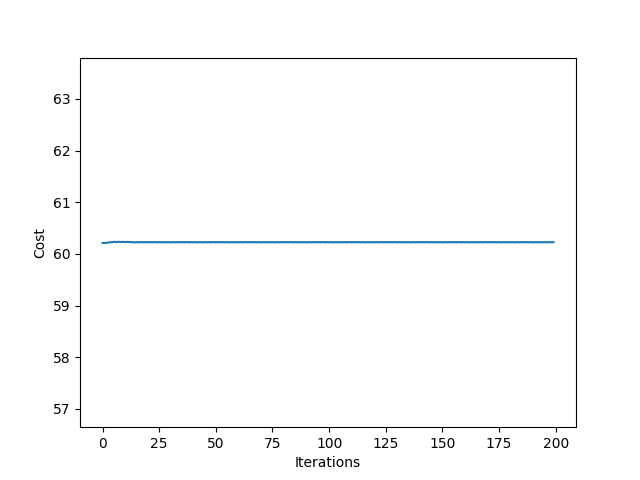
\includegraphics[scale=0.55]{fig_1.png}
    
    $\alpha = 1.0$
    
    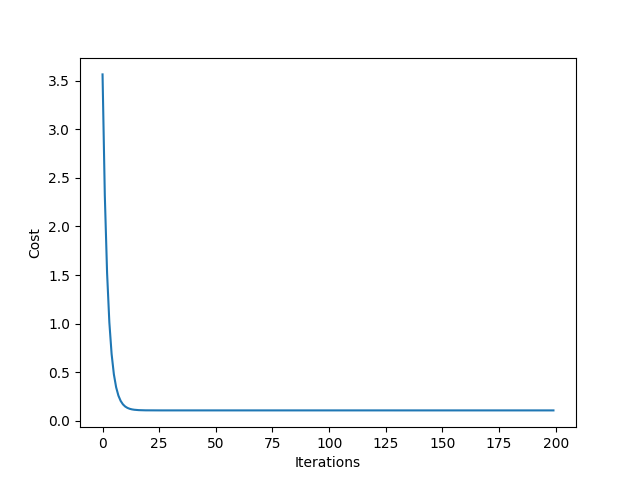
\includegraphics[scale=0.55]{fig_2.png}
    
    $\alpha = 0.1$
    
    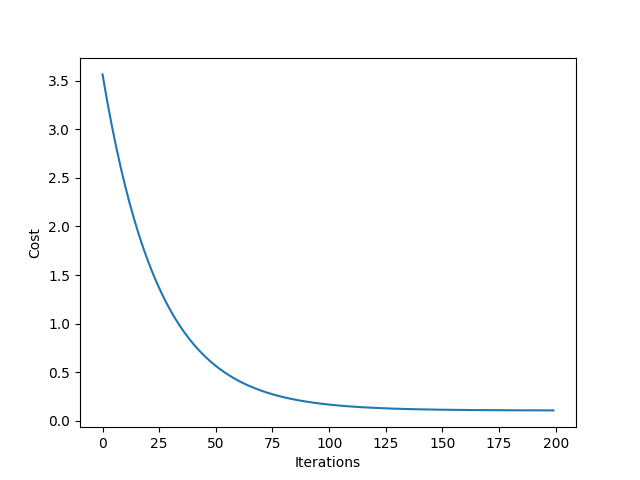
\includegraphics[scale=0.55]{fig_3.png}
    
    $\alpha = 0.01$
    
    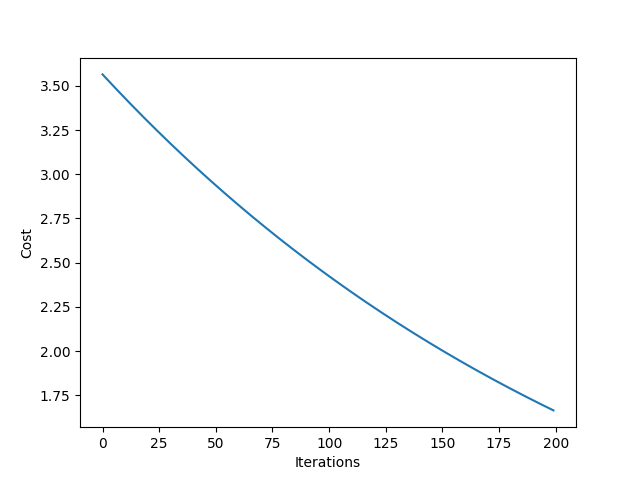
\includegraphics[scale=0.55]{fig_4.png}
    
    $\alpha = 0.001$
    
\end{center}

It is evident from the above plots that $\alpha = 0.1$ is the optimal learning rate as it arrives at suitable parameter values in fewer than 15 iterations. The plot for $\alpha = 1.0$ shows that this learning rate is much too high as no convergence will ever occur. The two remaining plots take too long to converge on optimal parameter values (with $\alpha = 0.001$ not even converging at all after $200$ iterations).

\noindent (ii) The parameter values, $\theta_0, \theta_1$, for each value of $\alpha$ are as follows:

\begin{center}
    \begin{tabular}{|c|c|c|}
        \hline
        $\alpha$ & $\theta_0$ & $\theta_1$ \\
        \hline
        $1.0$ & $0.608$ & $-0.812$ \\
        $0.1$ & $0.000$ & $0.945$ \\
        $0.01$ & $0.011$ & $0.914$ \\
        $0.001$ & $0.407$ & $-0.232$ \\
        \hline
    \end{tabular}
\end{center}

These values are consistent with the plotted values of $J(\theta)$ from the previous question: $\alpha = 1.0$ does not converge at all while neither $\alpha = 0.01$ or $\alpha = 0.001$ converge on the optimal parameter values fast enough. Once again, $\alpha = 0.1$ appears to be the optimal choice in this case.

\noindent (iii) The cost function at the final iteration for $\alpha = 0.1$ (the optimal learning rate) is $0.107$. Using the \texttt{part\_iii()} method in the code we can produce a scatter plot containing our normalised input and output variables. This results in the following graph:

\begin{center}
    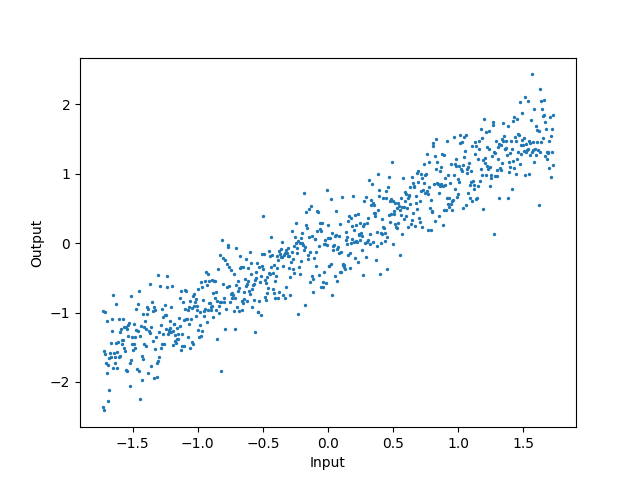
\includegraphics[scale=0.6]{fig_5.png}
\end{center}

Since we want predict a constant value, $v$, we will need to select a model of the form $y = 0x + v$. We will try to select $v$ such that there are an equal number of points above and below the line $y = v$. Since our normalised data has a mean of $0$ we know that the line $y = 0$ will produce the best result (this is also intuitively evident from the above graph). Running the cost function, $J(\theta)$ with $0$ for both of our parameter values returns the following result: $1.000$. This is significantly larger than the final cost of our trained model as is to be expected.

\noindent (iv) The \texttt{part\_iv()} method in the code uses SciKit's \texttt{StandardScaler} to normalise the input and output variables and \texttt{LinearRegression} to train the model. This model results in an intercept ($\theta_0$) of $0.000$ and a coefficient ($\theta_1$) of $0.945$. Theses results are identical to those found in (i) for $\alpha = 0.1$ which indicates, once again, that this is the optimal learning rate out of those that were tested.

\section*{Appendix: Code}

\begin{lstlisting}[language=Python]
from random import uniform
from sklearn import linear_model, preprocessing
import matplotlib.pyplot as plt
import numpy as np
import pandas as pd

def normalise(data):
    # normalise using the mean and standard deviation
    mu = sum(data) / len(data)
    sigma = (sum(pow(d - mu, 2) for d in data) / len(data)) ** 0.5
    return list(map(lambda d: (d - mu) / sigma, data))

def h(theta_0, theta_1, x):
    return theta_0 + (theta_1 * x)

def J(theta_0, theta_1, X, Y):
    M = len(X)
    return sum(pow(h(theta_0, theta_1, X[i]) - Y[i], 2) for i in range(M)) / M

def gradient_descent(X, Y, alpha, theta_0, theta_1):
    M, ITERATIONS = len(X), 200
    costs = [None] * ITERATIONS
    for i in range(ITERATIONS):
        costs[i] = J(theta_0, theta_1, X, Y)
        theta_0 += -2 * alpha / M * sum(h(theta_0, theta_1, X[i]) - Y[i]
            for i in range(M))
        theta_1 += -2 * alpha / M * sum((h(theta_0, theta_1, X[i]) - Y[i]) * X[i]
            for i in range(M))
    return costs, theta_0, theta_1

def part_i(data):
    X = normalise([d[0] for d in data])
    Y = normalise([d[1] for d in data])
    # randomly select starting parameter values
    start_theta_0, start_theta_1 = uniform(-1, 1), uniform(-1, 1)
    for alpha in [1.0, 0.1, 0.01, 0.001]:
        costs, theta_0, theta_1 = gradient_descent(X, Y, alpha,
            start_theta_0, start_theta_1)
        print(
            'alpha = %.3f >> theta_0 = %.8f, theta_1 = %.8f, cost = %.8f' %
            (alpha, theta_0, theta_1, costs[-1])
        )
        plt.plot(costs)
        plt.xlabel('Iterations')
        plt.ylabel('Cost')
        plt.show()

def part_iii(data):
    X = normalise([d[0] for d in data])
    Y = normalise([d[1] for d in data])
    plt.scatter(X, Y, s=2)
    plt.xlabel('Input')
    plt.ylabel('Output')
    plt.show()

def part_iv(data):
    X = np.array([d[0] for d in data]).reshape(-1, 1)
    X = preprocessing.StandardScaler().fit_transform(X)
    Y = np.array([d[1] for d in data]).reshape(-1, 1)
    Y = preprocessing.StandardScaler().fit_transform(Y)
    model = linear_model.LinearRegression().fit(X, Y)
    print(
        'theta_0 = %.8f, theta_1 = %.8f' %
        (model.intercept_, model.coef_)
    )

data = pd.read_csv('dataset.csv', comment='#').values.tolist()
part_i(data)
part_iii(data)
part_iv(data)
\end{lstlisting}

\end{document}
